\chapter{Local Automatic Differentiation}
\label{ch:LocalAD}
This chapter will consider a different approach on how to use AD to solve PDEs. When solving PDEs using a finite element method each cell will only depend on the neighbouring cells. In the \texttt{FAD} and \texttt{CJAD} implementations, the dependencies are stored in the discrete gradient and divergence operators. The implementation of \texttt{FAD} and \texttt{CJAD} calculates the residual function value and corresponding Jacobian for the whole grid simultaneously by having a vector to store the values and sparse matrices for the Jacobians. Hence when the discrete gradient and divergence operators are used in the calculation of the residual function in \autoref{ch:FlowSolver}, the Jacobian are automatically obtained with the structure seen in \autoref{fig:flowSolverJacobian}. However, this structure is known from the grid properties given in the \texttt{G} variable introduced in \autoref{sec:GridConstruction}. So instead of calculating the residual function for all cells at once, the new approach takes one cell at the time and sums up the contributions from each neighbour. This is done for each cell until all the residual functions for each cell is calculated. This new approach is called local AD and the method is based on the same idea as how AD is done in OPM \emph{\citep{OPM}}. Since OPM is written in C and C++ it is interesting to see if you can write similar type of code in Julia and obtain the same computational efficiency. \todo{Må teste noe mot dette og kommentere for at dette skal kunne stå der}

\section{Implementation}
\label{sec:LADImplementation}
To get a better understanding of how Local AD works, it is best to look at how it is implemented. Like for \texttt{FAD} and \texttt{CJAD} I have implemented local AD using a struct called \texttt{LAD}:
\lstinputlisting{code/LAD_structSimple.jl}
Since we now only operate on one cell at the time the implementation of local AD is simpler than for \texttt{FAD} and \texttt{CJAD}. The value of the AD-variable is now only a scalar and the Jacobian matrices is replaced by a vector of derivatives. These are the derivatives  with respect to the primary variables in the cell. To easily create a new \texttt{LAD} primary variable with a given number of derivatives and where the derivative with respect to itself is $1.0$, I have created a function called \texttt{createVariable}:
\lstinputlisting{code/createVariable.jl}
For the single phase flow solver in \autoref{ch:FlowSolver}, the derivatives vector will be of length one, as each cell only contain one primary variable (pressure). The implementation of \texttt{LAD} is however with \texttt{derivatives} as a vector. This is for the opportunity to implement more complex simulations like a two or three phase simulation where each cell can contain water, oil and/or gas \todo{legg til referanse her om to-fase simulering blir vellykket}. The implementation of operators for the \texttt{LAD} struct is done similar as explained in \autoref{ch:Implementation} for \texttt{FAD} and \texttt{CJAD}, but since we only have a vector of derivatives instead of a Jacobian matrix, the implementation is easier and follows the lines of the description from \autoref{sec:FADWithMultipleParameters}. 

Where the implementation of the local AD tool is easier than for \texttt{FAD} and \texttt{CJAD}, there is more work when calculating the residual functions. Since we do not use discrete gradient and divergence operators, but traverse through the grid cell by cell, we need somewhere to store the resulting values of the residual function. We also need a method to traverse through all the cells and to calculate the contributions from each neighbouring cell. Where the AD part of the code in \texttt{FAD} and \texttt{CJAD} were fully separated from the simulation, for local AD it is more integrated. This means that when using local AD to create the simulation it becomes a more application specific implementation than the method for \texttt{FAD} and \texttt{CJAD}. To create the flow solver from \autoref{ch:FlowSolver} I have chosen to store the calculated values of the residual functions in another struct called \texttt{FlowSystem}:
\lstinputlisting{code/FlowSystem.jl}
This struct look very similar to the other AD structs, except from \texttt{globalJac} being one single sparse matrix instead of a vector of sparse matrices and each element in \texttt{globalJac} being a vector. At this point you might not understand why it is quicker to calculate the residuals cell by cell compared to everything in one go. The key reason for this is that we know that the structure of the global Jacobian will stay the same throughout the whole simulation. This means we can use the grid variable \texttt{G}, that contains the information on which cells are neighbours, and build the correct structure of \texttt{globalJac} once and for all. When we run the simulation we only change the values inside of \texttt{globalJac}, but the structure stays the same. This reuse of \texttt{globalJac} will save a lot of memory allocations and hence speed compared to \texttt{FAD} and \texttt{CJAD} which allocates new structs for each calculation. By creating a new constructor for \texttt{FlowSystem} that uses the grid variable \texttt{G}, the variables \texttt{eqVal} and \texttt{globalJac} will be allocated with the correct length and the correct structure before the simulation begins. For the grid in \autoref{ch:FlowSolver} we have 1000 cells. This implies 1000 different pressure values and in addition we have the bottom-hole pressure (\texttt{bhp}) and the total production (\texttt{qS}). Hence \texttt{eqVal} will be a vector of length 1002.

Now that \texttt{FlowSystem} stores the  values and Jacobian of the residual functions, we need a new function to traverse through all cells and performing the calculations. I have chosen to call this function \texttt{assembleFlowSystem!()} where the exclamation mark is a Julia convention for a function that modifies its input parameters. The code for \texttt{assembleFlowSystem!()} can be seen below. I have removed all declarations of help variables and replaced the code for updating \texttt{FlowSystem} with comments to highlight the important parts of the function structure.
\lstset{numbers=left}
\lstinputlisting{code/assembleFlowSystem!.jl}
\lstset{numbers=none}
The input parameter \texttt{well} is a struct that contains all necessary information about the well. The first line in \texttt{assembleFlowSystem!()} resets \texttt{eqVal} and \texttt{GlobalJac} such that the structures are unchanged, but all the values are zero. Then the function begin traversing through the grid and for every cell it iterates through all neighbouring cells. Be aware that the looping variable names \texttt{fromCell} and \texttt{toCell} can be a bit misleading when they represent bottom-hole-pressure and total production, as those primary variables do not belong to any cell. The \texttt{eqVal} and \texttt{globalJac} variables are updated in line number 6, 8 and 10 inside the inner loop. As a reminder, the residual functions that \texttt{FlowSystem} eventually will represent are the functions \texttt{presEq}, \texttt{rateEq} and \texttt{ctrlEq} defined in \autoref{sec:setupGovEq}:
\lstinputlisting{code/governingEquationsPresSolver.jl}
In line number 6, \texttt{fromCell} and \texttt{toCell} are equal, but not the bottom-hole-pressure or total production. Here the first term in the sum in \texttt{presEq}, or the backward Euler term, is calculated. This is performed in an outer function called \texttt{timeDerivative()} that returns a \texttt{LAD} struct:
\lstinputlisting{code/timeDerivative.jl}
In \texttt{FAD} and \texttt{CJAD} we made all the primary AD-variables before the simulation. We then used them as input parameters in the residual functions that returned new AD-variables which represented the values and Jacobians. With local AD we create new primary AD-variables for the applicable cell inside the function we want to evaluate. For \texttt{timeDerivative()} we create a \texttt{LAD} primary variable that represent the pressure in the cell before we calculate the backward Euler term. When \texttt{timeDerivative()} have returned the new \texttt{LAD} variable, \texttt{assembleFlowSystem!()} adds the calculated value to the correct index in \texttt{eqVal} and the derivative vector to the correct diagonal index in \texttt{globalJac}.

In line number 10, when \texttt{fromCell} and \texttt{toCell} are two neighbouring cells, the divergence term in \texttt{presEq} is calculated. Like for \texttt{timeDerivative()}, we create the primary AD-variables inside the function, but since we calculate the flux from one cell to another we have to be careful with which direction we calculate the flux and which cell we want the derivative with respect to. Since the varying variables is named \texttt{fromCell} and \texttt{toCell} it is natural that the function \texttt{flux()}, seen below, calculates the flux from \texttt{fromCell} to \texttt{toCell}. 
\lstinputlisting{code/fluxFunctionLocalAD.jl}
What needs to be chosen is which cell we want the derivative with respect to. The choice only affect which indices of the Jacobian the calculated derivatives should be added or subtracted to. In \texttt{flux()} I have decided to calculate the derivative with respect to \texttt{fromCell}. The two first lines shows this result where \texttt{pFrom} is initialized with a derivative of $1$ and \texttt{pTo} as a constant. This choice leads to the following code for updating \texttt{FlowSystem} at line number 10 in \texttt{assembleFlowSystem!()}:
\lstinputlisting{code/fluxCodeLocalAD.jl}
The value of \texttt{fluxLAD} is added to \texttt{eqVal} and the derivative of the flux with respect to \texttt{fromCell} is added to \texttt{globalJac}. In addition we know that the flux from \texttt{fromCell} to \texttt{toCell} is the same, but with negative sign, as the flux from \texttt{toCell} to \texttt{fromCell}. This means that the derivative of the flux from \texttt{toCell} with respect to \texttt{fromCell} needs to be subtracted with \texttt{fluxLad.derivatives}. For a facet between two neighbours we will with \texttt{assembleFlowSystem!()} calculate the value of the flux through the facet twice, only with different signs. You might think that we could save time by subtracting \texttt{fs.eqVal[toCell]} with \texttt{fluxLAD.val}, but since we also will need the opposite derivatives of this particular flux, there will small, or next to none, computational gain of exploiting this fact. In worst case it might actually become a slower implementation, as we will have to keep track of which fluxes has been added to which cells. When the flux from all the neighbours has been added up for a cell, we have obtained the divergence in that cell. 

Line number 8 in \texttt{assembleFlowSystem!()} is the last line I have not commented and it is where the well equations, \texttt{rateEq} and \texttt{ctrlEq}, are handled. This is line is executed if both \texttt{fromCell} and \texttt{toCell} is either one of the cells containing a well, the bottom-hole pressure or the total production. The information on which cells fulfilling this condition lies in \texttt{well}. The calculation is performed by handling every case such that the correct residual function is calculated differentiated with respect to the correct variable and like for the fluxes, the resulting values and derivatives is added to \texttt{FlowSystem} at the correct indices. \todo{Vurdere om det går an å være litt mindre vag. Tror det fort kan bli ekstremt på detaljnivå.}

Summed up the calculation of the residual functions using local AD is based on two modules. The first is the actual AD tool with the \texttt{LAD} struct, and the second is \texttt{FlowSystem} which keeps track of the global system and what calculations should be performed by the AD tool. With this approach we lose some of the advantages using the other AD tools where the discrete residual functions looked very similar to the continuous case, like explained in \autoref{sec:setupGovEq}. The main structure of \texttt{assembleFlowSystem!()} will however be the same no matter what type of simulation, hence making modifications to the code, or building another simulation, will not demand a complete change of code structure. \todo{sjekk om dette ikke ble litt vagt litt senere.}

\section{Optimizing Local AD}
As explained in the beginning of this chapter, the main idea behind local AD is to reuse the Jacobian to save memory usage and extra memory allocations. The implementation given in \autoref{sec:LADImplementation} has however left out some small, but key parts of the implementation that will massively decrease the memory and speed usage. This is purely implementation specific differences that has been left out to make the introduction to local AD more clear. It will not change the theory behind using local AD to solve PDE's.

\subsection{Dynamic VS Static Arrays}
The difference between a dynamic array and a static array is that a dynamic array can be extended or shortened as much as you like while a static array has a fixed length. Using a static array will give computational gain concerning speed and memory allocations compared to a dynamic array. This is because the compiler knows that a static array has the given fixed length forever and hence it can allocate the exact memory needed in advance and hence optimize the machine code. With a dynamic array it does not know if the array will grow larger, or smaller and it is much harder to optimize the machine code. 

Julia has a package called \emph{\cite{StaticArrays}} that provides static arrays to the the built in arrays without the possibility for changing the size of the array. The package provides two types of vectors, \texttt{SVector} and \texttt{MVector}. Both are static vectors, but \texttt{MVector} is mutable, meaning the values inside the vector can be changed, where the values inside an \texttt{SVector} is final when the vector is defined. This makes SVector ideal for \texttt{LAD.derivatives} since when we perform operations on \texttt{LAD} variables, new \texttt{LAD} variables are returned. \texttt{MVector} is however optimal for the elements in the sparse matrix \texttt{FlowSystem.globalJac} as we know how long each element vector will be, but we want to be able to change the values inside each vector. 

When the implementation is changed to use static vectors it needs to know how long these vectors are. When building a simulation it is not a problem to say in advance how many derivatives we need and when the compiler knows this before compilation it can optimize the machine code. OPM solves this by creating a template class \todo{Legg til både kilde og sjekk formulering} such that the compiler always knows that for this simulation, the static array will always have this fixed length. This is important because we do not want to create \texttt{LAD} structs with different lengths for \texttt{LAD.derivatives} and we want all vectors in \texttt{FlowSystem.globalJac} to have that same length. If we define this clearly the compiler can optimize the machine code much better than if it does not know if for example some elements in \texttt{globalJac} suddenly will be allocated with a longer static mutable array. This will also make the implementation of the operators of \texttt{LAD} easier, as we know for certain that all \texttt{LAD} variables will have \texttt{derivatives} with the same length. The best implementation I have found for this in Julia is to declare a global constant variable in the local AD module such that the new implementation of \texttt{LAD} becomes:
\lstinputlisting{code/LAD_struct.jl}
One disadvantage with this implementation is that the Local AD module needs to be modified to work with simulations with more primary variables for each cell. \todo{Må se om det finnes noen annen måte, hvis ikke bør det kanskje kommenteres at det er litt krøkkete} The implementation of \texttt{FlowSystem} imports the local AD module, hence it can also use the global constant in the new implementation:
\lstinputlisting{code/FlowSystemFixed.jl}

\section{Flow Solver with Local AD}
\label{sec:flowSolverWithLAD}
Now that \texttt{FlowSystem} and \texttt{LAD} has been implemented with static arrays it is interesting to see how this method compares to \texttt{FAD} and \texttt{CJAD} in the simulation from \autoref{ch:FlowSolver}. Since OPM is a simulator ment to be much faster than MRST, it is assumed that since Julia is supposed to run as fast as C, the local AD approach will give a computational gain. With the implementation given in this chapter this is however not the case. It performs worse than \texttt{CJAD} and similar to \texttt{FAD}. As explained in \autoref{sec:profiling}, profiling is an efficient way of finding the bottlenecks in a code, and this is a perfect example of when to use it - the code was expected to be faster, but it was not, so it is important to find out if there is a small part of the code that is slow. \autoref{fig:profileSlowCreateVar} shows a screenshot of a profile result from running the flow solver simulation. The screenshot only contains blocks from the \texttt{flux} function. Two blocks are marked with squares and two other blocks with brighter diagonal stripes. The blocks with squares are time spent in \texttt{createVariable()} and the brighter diagonal stripes are AD calculations in \texttt{flux}.
\begin{figure}[H]
    \centering
    \begin{subfigure}[t]{0.75\textwidth}
        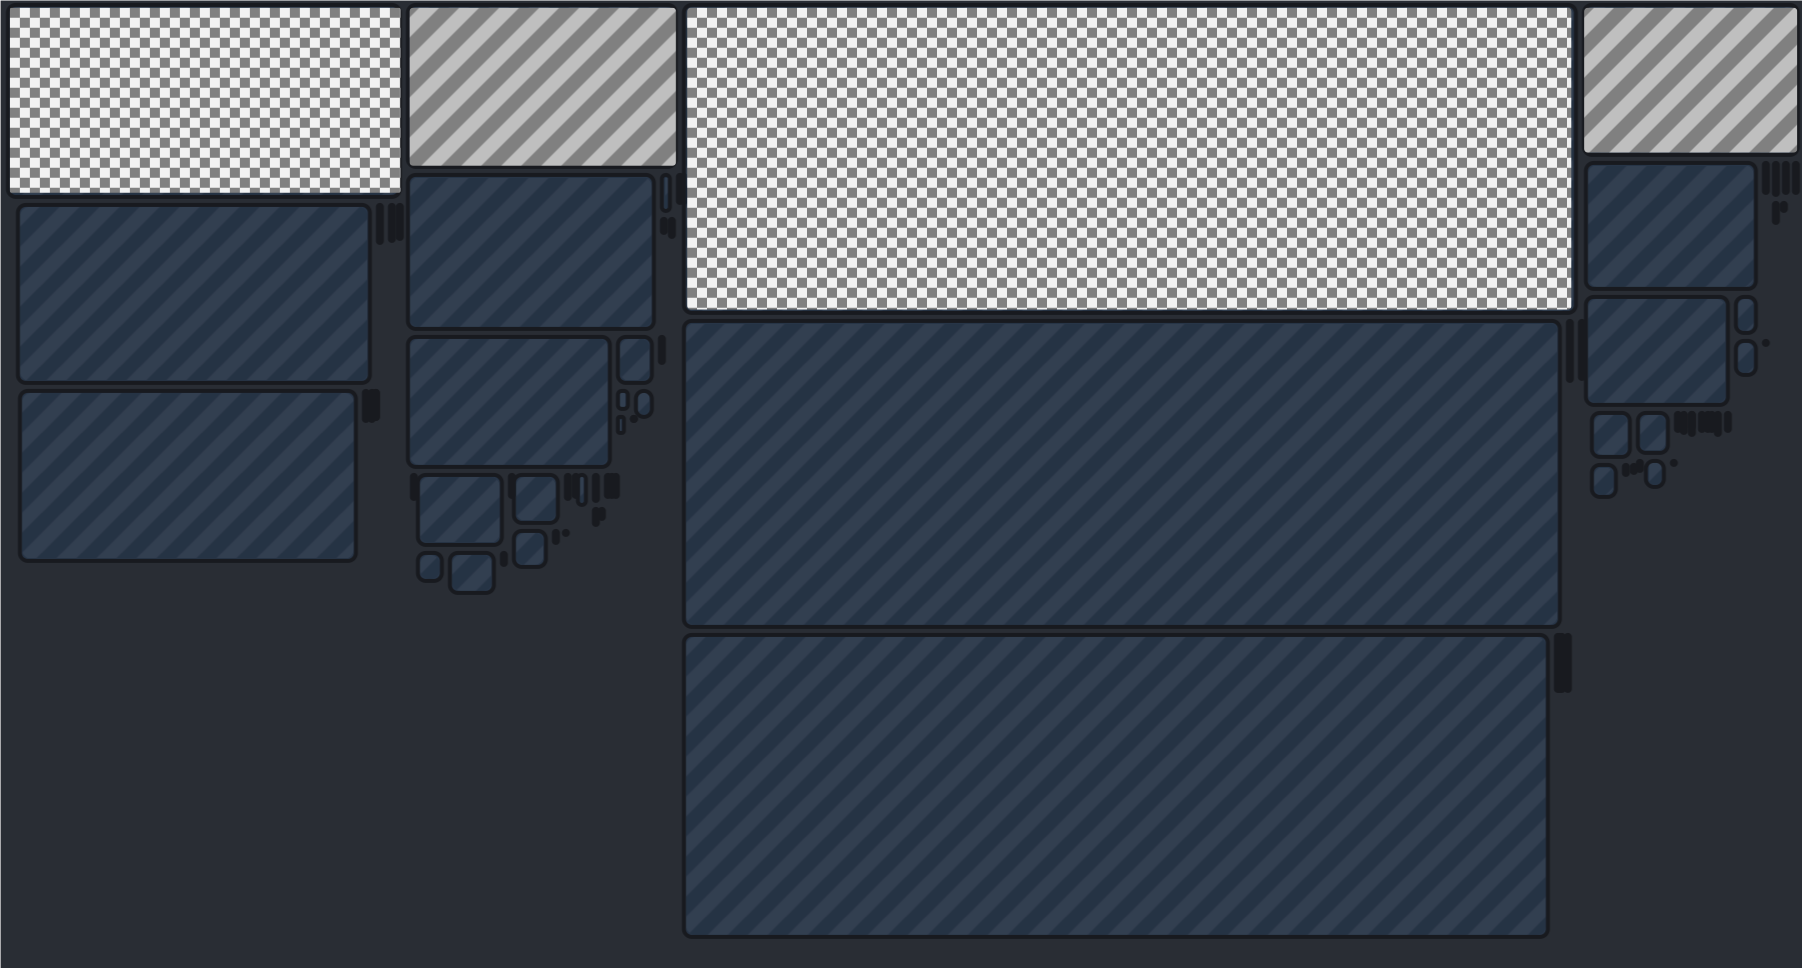
\includegraphics[height = 0.35\textheight, width=\textwidth ]{figures/profilingSlowCreateVariablesFlux.png}
        \caption{}
        \label{fig:profileSlowCreateVar}
    \end{subfigure}
    \hspace{0.06\textwidth}
    \begin{subfigure}[t]{0.18\textwidth}
        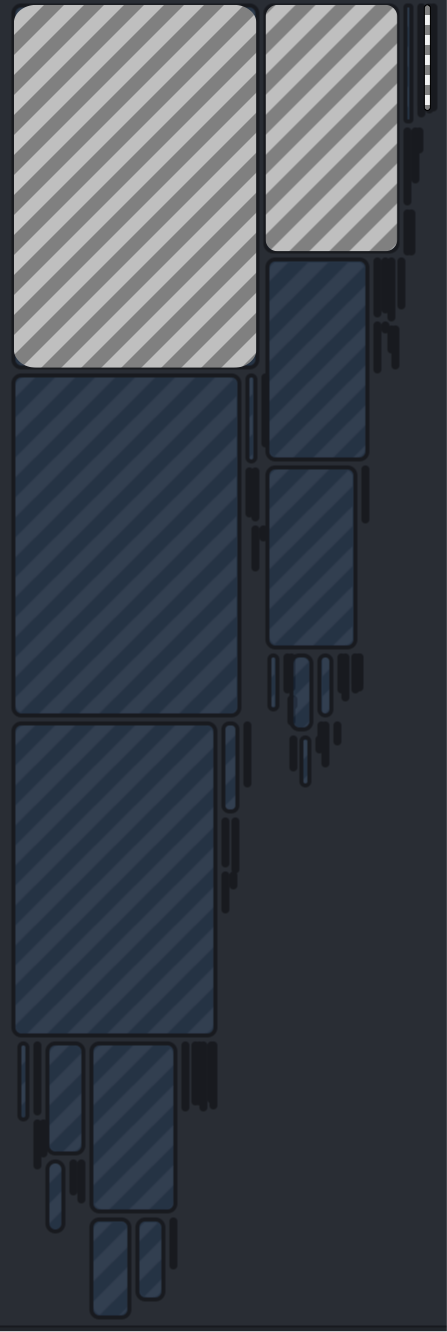
\includegraphics[height = 0.35\textheight, width=\textwidth]{figures/profilingFastCreateVariablesFlux.png}
        \caption{}
        \label{fig:profileFastCreateVar}
    \end{subfigure}
    \caption{The figures shows screenshots of the profile result from the \texttt{flux} function in the flow solver simulation from \autoref{ch:FlowSolver}. The blocks marked with squares are time spent in \texttt{createVariable()} and the blocks with bright diagonal lines are calculations in \texttt{flux}. \autoref{fig:profileSlowCreateVar} uses a slow version of \texttt{createVariable()} while \autoref{fig:profileFastCreateVar} uses a faster version.}
\end{figure}
It makes no sense that creating a \texttt{LAD} struct should take more time than the actual AD calculations. This indicates that the \texttt{createVariable()} function is poorly implemented. This is also the case as even though we only want to create a static \texttt{Svector}, we start by creating a dynamic vector of zeros, then we modify the vector by changing one of the values to one, and finally we convert the dynamic vector into a static \texttt{SVector}. The new implementation seen below is a much better implementation where the \texttt{SVector} is created immediately as the correct vector without any use of dynamic vectors.
\lstinputlisting{code/createVariableFast.jl}
The new profiling result with the updated \texttt{createVariable()} can be seen in \autoref{fig:profileFastCreateVar}


\todo[inline]{Se på parallellisering for lokal AD?}